% !TEX root = ../elsarticle-template.texmain.tex
%-------------------
\section{Problem Statement}
\label{sec:problemstatement}

%In this section, we describe the problem addressed in this article. To this end, we first describe the development scenario behind bottom-up language product lines. Then, we define the scope of our approach. %That means that the solution presented in this article is useful when the development project satisfies the constraints described in this scenario; other situations will need other type of solutions.

%\subsection{The Development Scenario: \\ \textbf{Bottom-Up Language Product Lines}}
\label{sec:thedevelopmentscenario}

Similarly to software product lines \cite{Linden:2007}, the development process of language product lines can be divided into two phases: domain engineering and application engineering. During the domain engineering phase, language designers build the language product line. This process includes the design and implementation of a set of interdependent language modules that implement the language features and the construction of variability models encoding the rules in which those features can be combined to produce valid DSL variants. During the application engineering phase, diverse DSL variants are derived according to specific needs. Such a derivation process comprises the selection of the features to include in a given DSL variant, i.e., language configuration and the assembly of the corresponding language modules, i.e., language modules composition.

%The top-down and bottom up approaches are two different ways to face the aforementioned phases. In the top-down approach, domain engineering is performed first and application engineering is performed afterwards. During domain analysis, language engineers use domain analysis techniques to design and implement a set of language modules and variability models from some domain knowledge owned by experts and final users. Those artifacts can be later used to configure and compose particular DSL variants in the application engineering phase.

Note, however, that in bottom-up language product lines, application engineering is performed first and domain engineering is performed afterwards through reverse-engineering techniques. During the application engineering phase, language designers build an initial DSL. As the language development project evolves, some DSL variants are needed to address new requirements. Language designers create new development branches where they implement these new variants with the corresponding adaptations. At some point, language designers realize that there is potential reuse among the variants. Hence, they launch a reverse engineering process --which in this case corresponds to the domain (re)engineering phase-- where the existing DSL variants are used to build up a language product line. Using this language product line, language designers can revisit the application engineering phase in order to create new DSL variants.

%\begin{figure*}
%	\centering
%	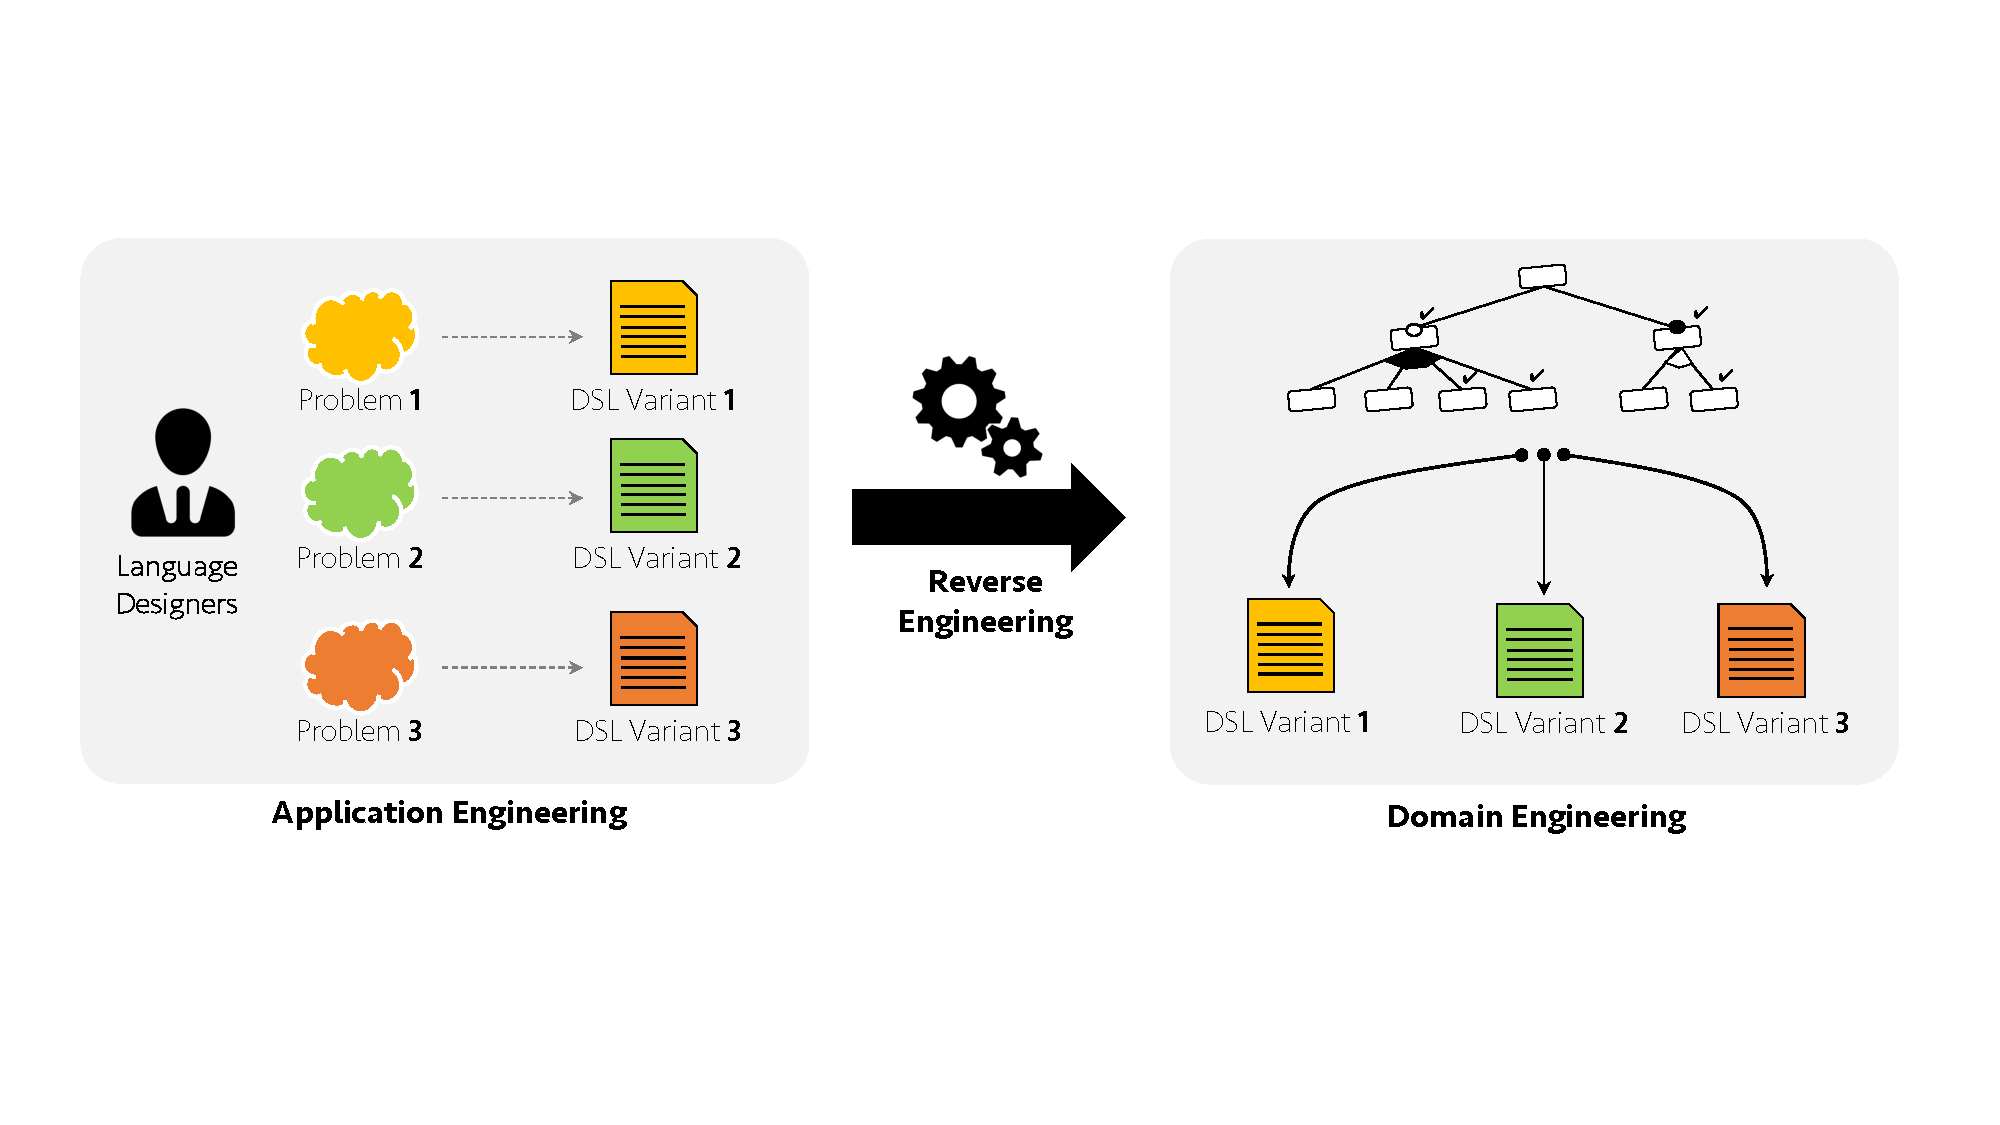
\includegraphics[width=0.8\linewidth]{images/bottom-up-lpl-fig.pdf}
%	\caption{Bottom-up language product lines engineering \label{fig:lple-dimensions}}
%\end{figure*}

%\vspace{2mm}
%\textit{\textbf{The clone-and-own approach.}} In this article, we are interested in bottom-up language product lines. Specifically, we propose a technique to reverse engineering language product lines from sets of existing DSL variants built through the \textit{clone-and-own} approach. With this approach, DSL variants are created by cloning existing versions of a DSL and performing certain adaptations intended to satisfy a specific purpose. While several research works have shown that the clone-and-own practice is common in software development projects \cite{Mayrand:1996,Rubin:2015}, in a recent work we provided empirical evidences that show that it is also a common practice during language development \cite{MendezAcuna:2016}. We conducted an analysis of a large pool of DSLs obtained from \texttt{GitHub}, and we detected a relevant amount of specification clones among them. You can found the sources of the experiments in a dedicated web-site\footnote{\url{http://empiricalpuzzle.weebly.com/}}.

%As a response to this phenomenon, recent research works have proposed mechanisms to reverse engineering software product lines from sets of existing software products which share code clones. This type of approaches are a clear example of bottom-up software product lines. and discussed its on software maintenance \cite{Chatterji:2016}

%Another important characteristic of the development process during the construction of bottom-up language product lines is that, in many cases, language designers use the copy/paste/modify pattern to create  individual DSLs. This approach is explained by Lopez Herrej\'on et all for the general case of software product lines.

\subsection{Motivating scenario} Suppose a team of language designers working on the construction of the DSL for finite state machines. Initially, language designers followed the UML specification \cite{UML:2011} to define language constructs such as states, regions, transitions, and triggers. Those language constructs are specified in terms of their syntax and semantics. So, at the end of the language development process, language designers release an executable DSL which behavior complies the UML specification.

Once this first DSL was released, the language designers are asked to build a new variant which must comply the Rhapsody specification \cite{Harel:2004} (i.e., another formalism to finite state machines). This new variant shares many commonalities with UML state machines, but introduces differences at both syntax and semantics levels \cite{Crane:2007}. After building this second variant, language designers obtained two different DSLs implementing different formalisms of state machines. Those DSL variants have some commonalities among them. And at the same time, the DSL have some particularities that make them unique.

Note that this process is repeated each time language designers have to build a new variant of the DSL for each new FSM formalism (e.g., Stateflow \cite{Martaj:2010} or Harel state machines \cite{Harel:1996}). This becomes specially challenging when final users need to combine some specifications to define hybrid formalisms. While several approaches have been proposed to reverse engineering software product lines from existing product variants \cite{LopezHerrejon:2015,Martinez:2015,Martinez:2015b}, in this article we propose techniques to reverse engineering language product lines from existing DSL variants.

\subsection{Scope: \textbf{Executable Domain Specific Languages}}
\label{sec:technologicalscope}

All the ideas presented in this article are focused to executable domain specific modeling languages (xDSMLs) where the abstract syntax is specified through \textit{metamodels}, and the dynamic semantics is specified operationally as a set of \textit{domain specific actions} \cite{Combemale:2013}. Whereas metamodels are class diagrams that represent language constructs and relationships among them, domain specific actions are Java-like methods that introduce behavior in the metaclasses of a given metamodel \cite{Jezequel:2015b}. 

Fig. \ref{fig:fig-dsl-example} illustrates this type of DSLs through a simple example on finite states machines. In that case, the metamodel that implements the abstract syntax contains three metaclasses: \textsl{StateMachine}, \textsl{State}, and \textsl{Transition}. There are some references among those metaclasses representing the relationships existing among the corresponding language constructs. The domain specific actions at the right of the Fig. \ref{fig:fig-dsl-example} introduce the operational semantics to the DSL. In this example, there is one domain specific action for each metaclass. Note that the interactions among domain specific actions can be internally specified in their implementation by means of the \textit{interpreter pattern}, or externalized in a model of computation \cite{Combemale:2013}.

\begin{figure}
\centering
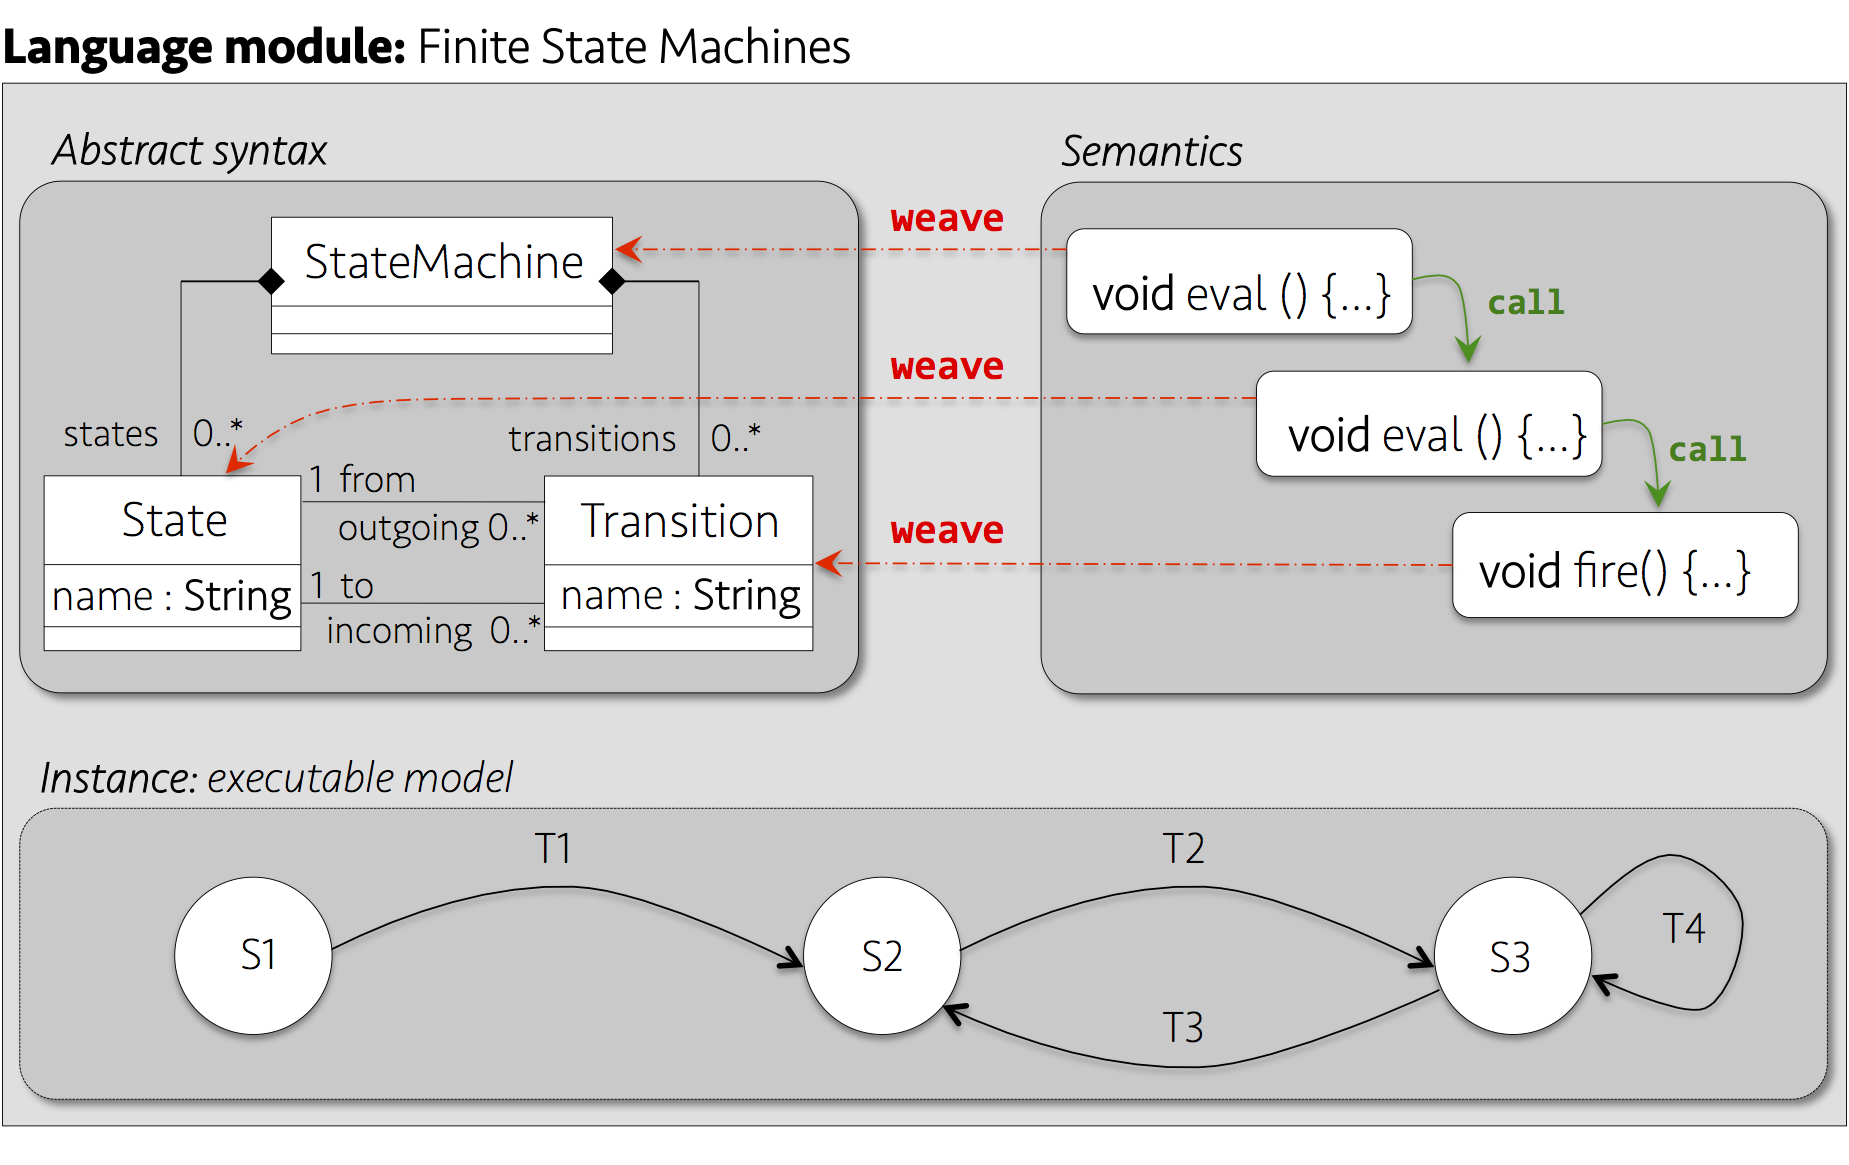
\includegraphics[width=1\linewidth]{images/fig-dsl-example.png}
\caption{A simple DSL for finite state machines}
\label{fig:fig-dsl-example}
\end{figure}
